\section{Restoring the Veto}
\label{sec:gate}

\begin{table}[t]
    \centering
    \small
    \setlength{\tabcolsep}{3pt}
    \resizebox{\columnwidth}{!}{\begin{tabular}{@{}llcccc@{}}
\toprule
Gate & Status & False-pos.\ episodes (\%) & Drop (\%) & mIoU & mIoU cost \\
\midrule
\multicolumn{6}{@{}l}{\emph{LVIS selection images (500)}} \\
none & -- & 99.8 & -- & 0.866 & -- \\
multiplicative & pre-reg., \textbf{fails} & 1.5 & 98.5 & 0.810 & 0.056 {\scriptsize[0.038, 0.077]} \\
hard, $\tau\!=\!0.10$ & post hoc & 5.7 & 94.3 & 0.861 & 0.005 {\scriptsize[0.000, 0.011]} \\
\multicolumn{6}{@{}l}{\emph{LVIS held-out images (500)}} \\
none & -- & 99.5 & -- & 0.864 & -- \\
hard, $\tau\!=\!0.10$ & pre-reg., passes & 6.4 {\scriptsize[5.1, 7.8]} & 93.6 & 0.862 & 0.002 {\scriptsize[0.000, 0.006]} \\
geometry & pre-reg., \textbf{fails} & 51.8 {\scriptsize[47.9, 55.9]} & 48.0 & 0.864 & 0.000 {\scriptsize[0.000, 0.000]} \\
\bottomrule
\end{tabular}
}
    \caption{\textbf{Gates on the exemplar pass.}
    False positives: absent phrase plus anchor box returns a mask.
    mIoU: consistent prompts, where the phrase names the anchor's category.
    Preregistered bars: a relative drop of at least 80\% and a cost of at most 0.03 (selection) or 0.02 (held-out).}
    \label{tab:gates}
\end{table}

\begin{figure}[t]
    \centering
    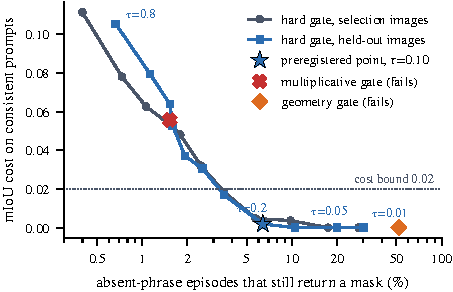
\includegraphics[width=\linewidth]{fig/gate.pdf}
    \caption{\textbf{Operating curve of the hard gate.}
    Each point is a threshold $\tau$ on the text-only presence probability.
    The star is the preregistered held-out result; the rest of both curves is computed after the fact from stored outputs.}
    \label{fig:gate}
\end{figure}

The text-only pass still rejects absent phrases (\cref{tab:veto}), and it shares the image features with the exemplar pass.
We therefore run the phrase once without the exemplar, read its presence probability $\ptext = \sigma(\spres^{\mathrm{text}})$, and use it to gate the exemplar pass.
The extra cost is one pass of the layers after the image backbone; the backbone is not run again.

\paragraph{Three gates.}
The \emph{multiplicative} gate substitutes $\ptext$ for the exemplar pass's own presence in \cref{eq:score}.
The \emph{hard} gate leaves \cref{eq:score} alone and discards the whole output when $\ptext < \tau$.
The \emph{geometry} gate is a softer hard gate: when $\ptext < \tau$ it still keeps masks whose IoU with the exemplar's rectangle is below 0.5, on the idea that the false output is the boxed region and other masks may be real.

\paragraph{The multiplicative gate fails on cost.}
This was our first design, and phase 1 passed it on COCO (false positives 99.9\% $\to$ 1.9\%, mIoU 0.809 $\to$ 0.793).
On LVIS phrases it removes the false positives, 99.8\% $\to$ 1.5\%, but costs 0.056 mIoU [0.038, 0.077] on consistent prompts against a bar of 0.03 (\cref{tab:gates}).
The cause is that text alone is not a reliable witness for present concepts in a 1,203-category vocabulary.
The text-only presence is non-negative for 92.0\% of present, exhaustively annotated categories (92.9\% of frequent ones, 77.0\% of the 61 common ones).
For 6.2\% of consistent prompts it is negative, and those prompts had an ungated mIoU of 0.860: the gate threw away good masks.

\paragraph{The hard gate at a low threshold passes.}
A present concept whose text-only presence is negative is usually not far below zero, while absent phrases are far below (\cref{fig:presence}).
Sweeping $\tau$ on the stored selection outputs, $\tau = 0.10$ leaves 5.7\% false positives at a cost of 0.005.
We fixed $\tau = 0.10$ and the bars, then ran the held-out images.
False positives fall from 99.5\% to 6.4\% [5.1, 7.8], a relative drop of 93.6\%, and mIoU moves from 0.864 to 0.862, a cost of 0.002 [0.000, 0.006].
The gate rejects one of the 500 consistent prompts.
The count of returned instances is as accurate as before (mean absolute error against the number of ground-truth instances 0.708 $\to$ 0.710).
The remaining 6.4\% are the absent phrases whose text-only presence probability is at least 0.10; the gate can be no better than the text-only head at that threshold.
\Cref{fig:gate} shows the trade-off: lowering $\tau$ to 0.05 costs nothing on the held-out images and leaves 10.5\%, and raising it to 0.5 leaves 1.6\% at a cost of 0.053.

\paragraph{The geometry gate fails on strength.}
It costs nothing on consistent prompts and removes only 48.0\% of the false positives, leaving 51.8\% [47.9, 55.9].
The false mask is the object inside the box, not the box, and an object's mask often has an IoU below 0.5 with its own bounding rectangle, so the rule keeps it.

\paragraph{When the gate is the wrong tool.}
A user adds an exemplar when text alone fails, and that is where a text-only gate is least reliable.
At $\tau = 0.10$ the text-only pass still admits 98.9\% of present frequent categories and 92.3\% of the 52 common ones on the held-out images.
There are five rare ones, too few to say anything.
For concepts the text encoder does not know, the gate should be off, which returns the model to its ungated behaviour.
\sam{} already has this switch in spirit: the paper notes that presence can be set to one when the concept is known to be present~\cite{carion2026sam3}.
The exemplar, in effect, sets it to one without being asked.
